\documentclass{article}
\usepackage{graphicx}
\graphicspath{ {images/} }
 
\begin{document}

Aufgabe 14:
Unser Icon wurde fuer die App „Pokemon GO“ entwickelt. Dies ist ein kommendes Augmented Reality Spiel von Nintendo, bei dem man ueber eine Karte der Erde sieht, wo sich bestimmte Pokemon zurzeit aufhalten. Diese Pokemon lassen sich fangen, indem man zu ihrem Platz auf der Welt reist. Mit den gefangen Pokemon kann man anschließend gegen andere Spieler antreten.
Als Mittelpunkt des Icons haben wir den Pokeball gewaehlt, ein ikonisches Symbol im Pokemon-Kosmos. Wir haben die Standardfarben Weiß, Rot und Schwarz eines Pokeballs beibehalten und lediglich die untere Seite des Balls veraendert. Statt der normalen weißen Farbe ist dort eine Darstellung der Welt platziert, um die Augmented Reality der App zu vermitteln. Die Landmasse auf dem Ball ist der Teil von Japan, das Ursprungsland von Pokemon, der die Vorlage für die Welten der ersten beiden Generationen ist. Zu guter Letzt haben wir auf Grund des Namens unserer App den Ball mit einem „G“ umschlossen. Die orangene Farbe leitet sich von dem bekannten Pokemon Glumanda ab und harmoniert mit dem roten Teil des Pokeballs, da beide Farben warm sind. Die Landmasse und Seemasse haben das Gruen und Blau der anderen beiden Startpokemon der ersten Generation, Bisasam und Schiggy.
Folgende Groeßenverhaeltnisse in unserem Icon liegen dem Goldenen Schnitt zu Grunde:
-	Die Groeße des „G“s im Verhaeltnis zum Ball
-	Die Groeße des weißen Rings, der den schwarzen Ring umschließt im Verhaeltnis zum schwarzen Ring selbst

 
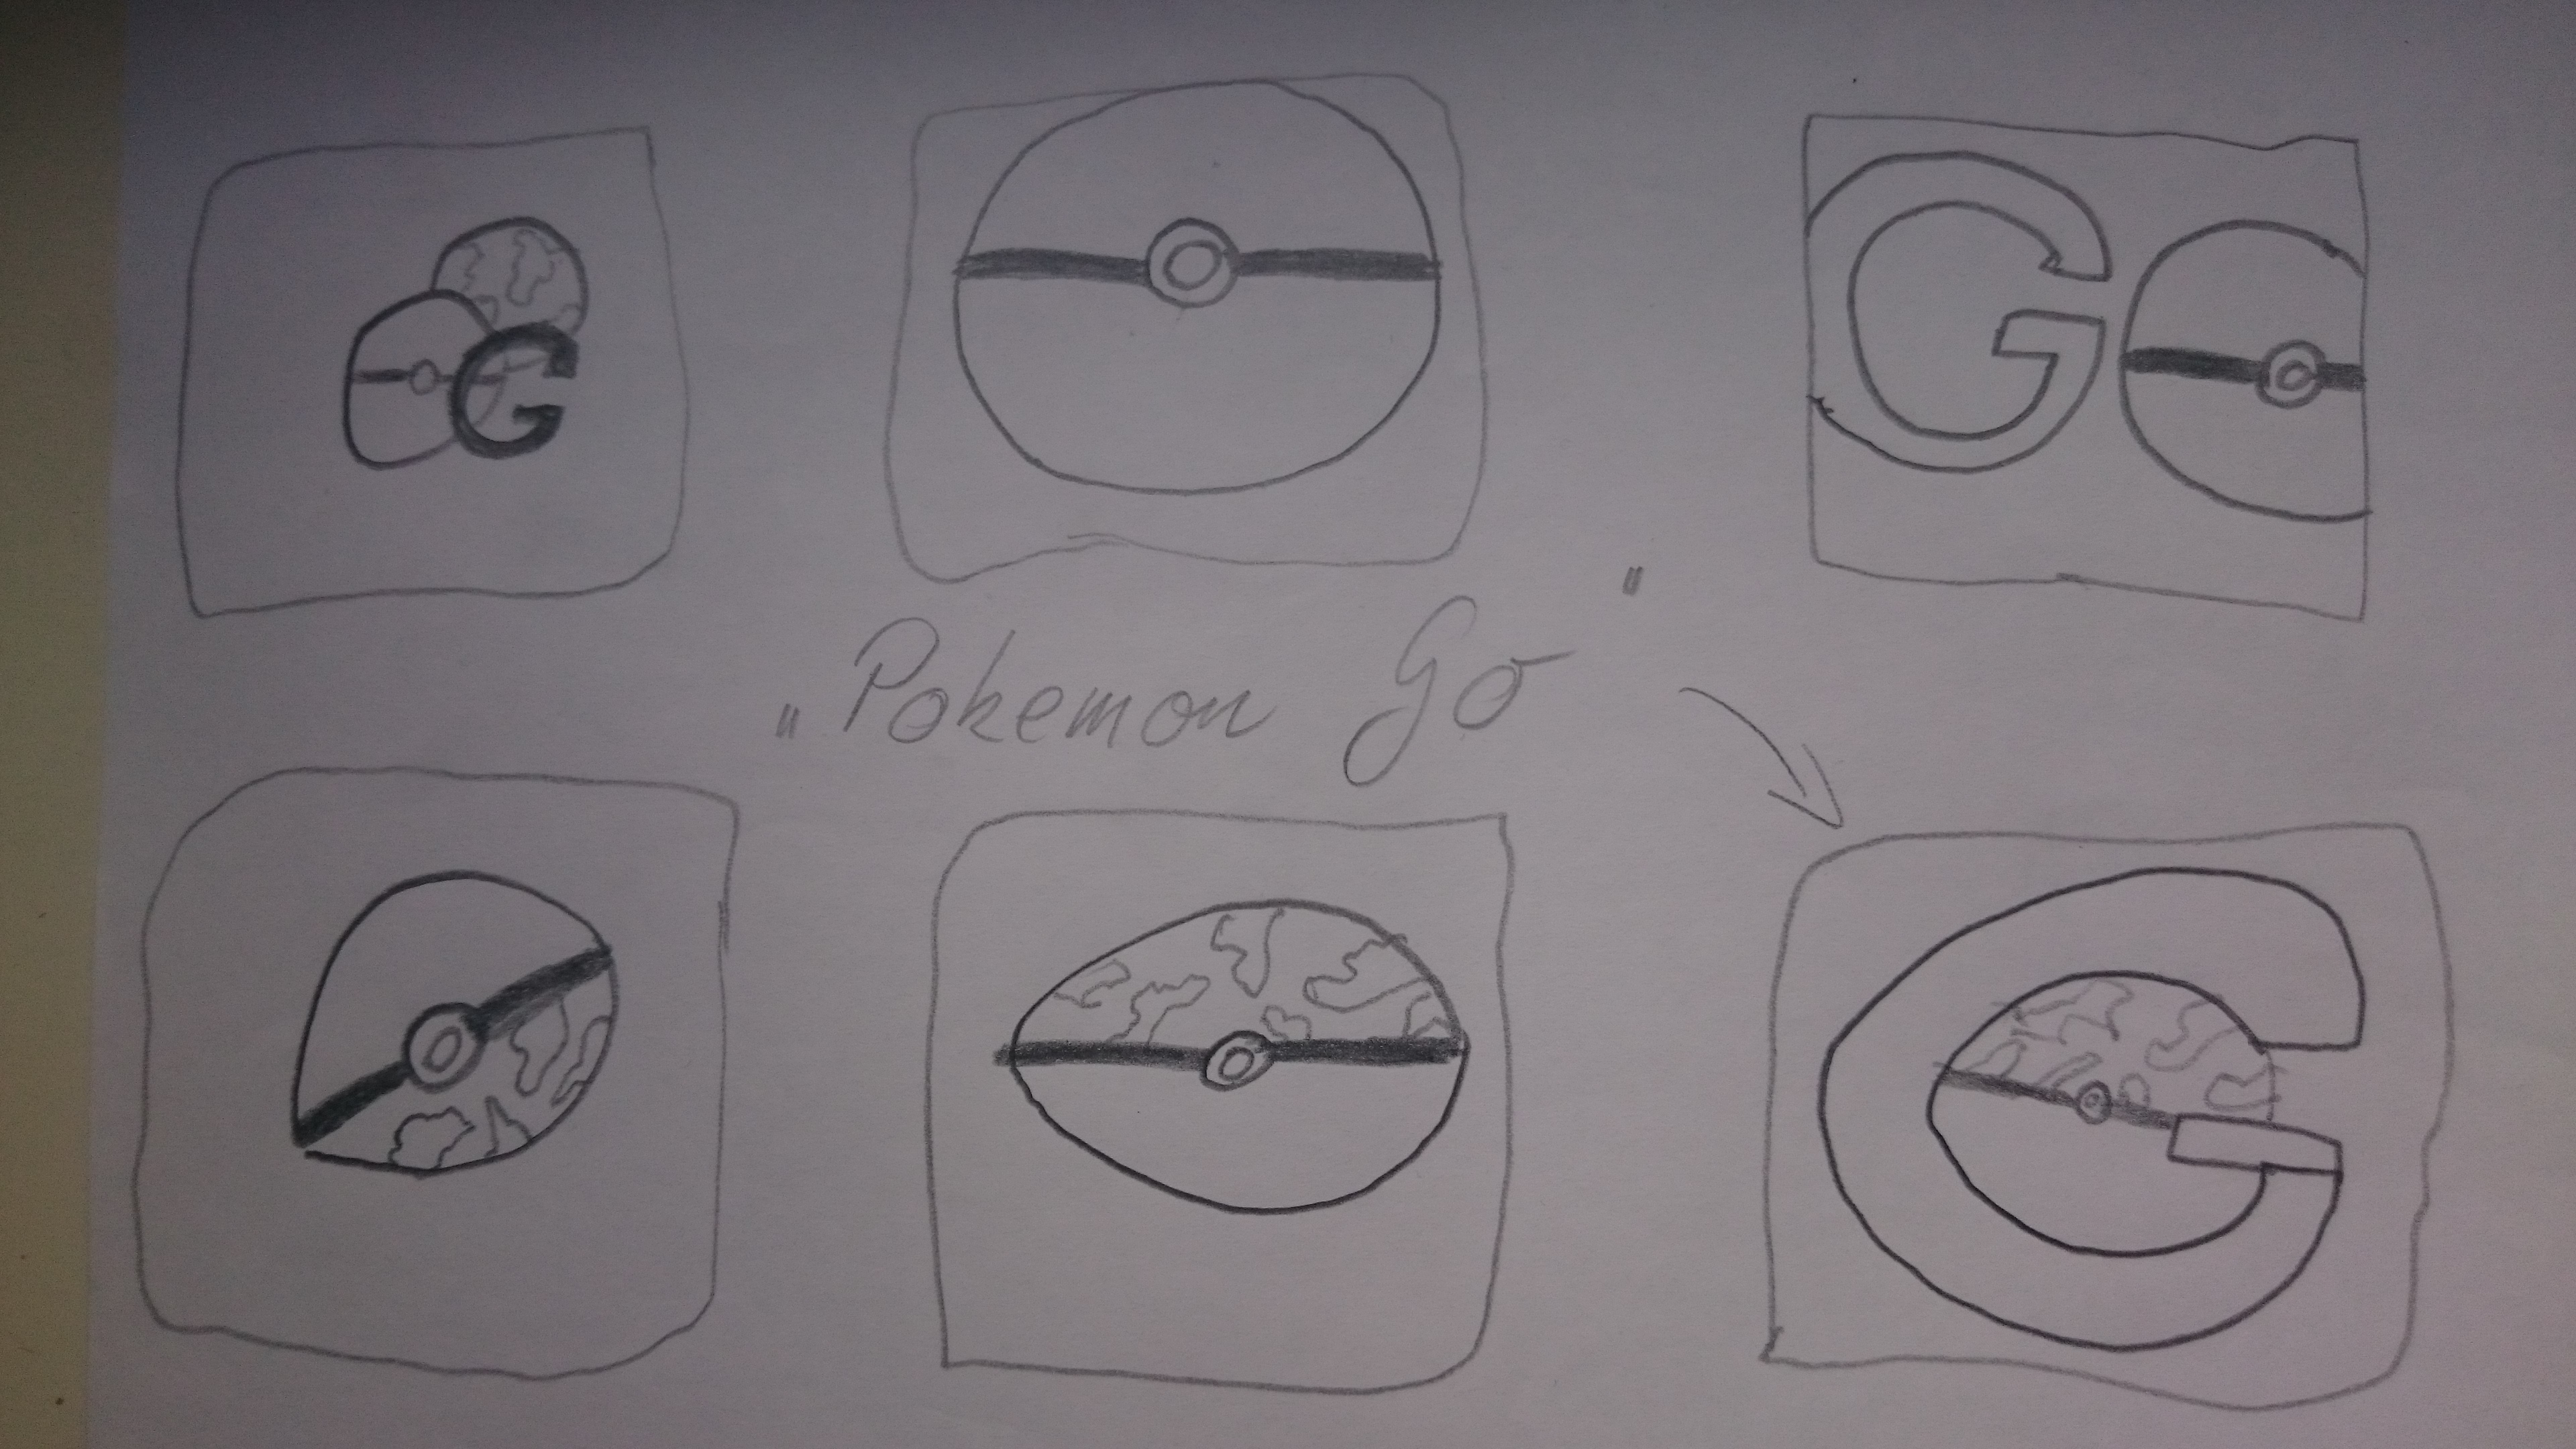
\includegraphics[scale=0.13]{DSC_0758.jpg}
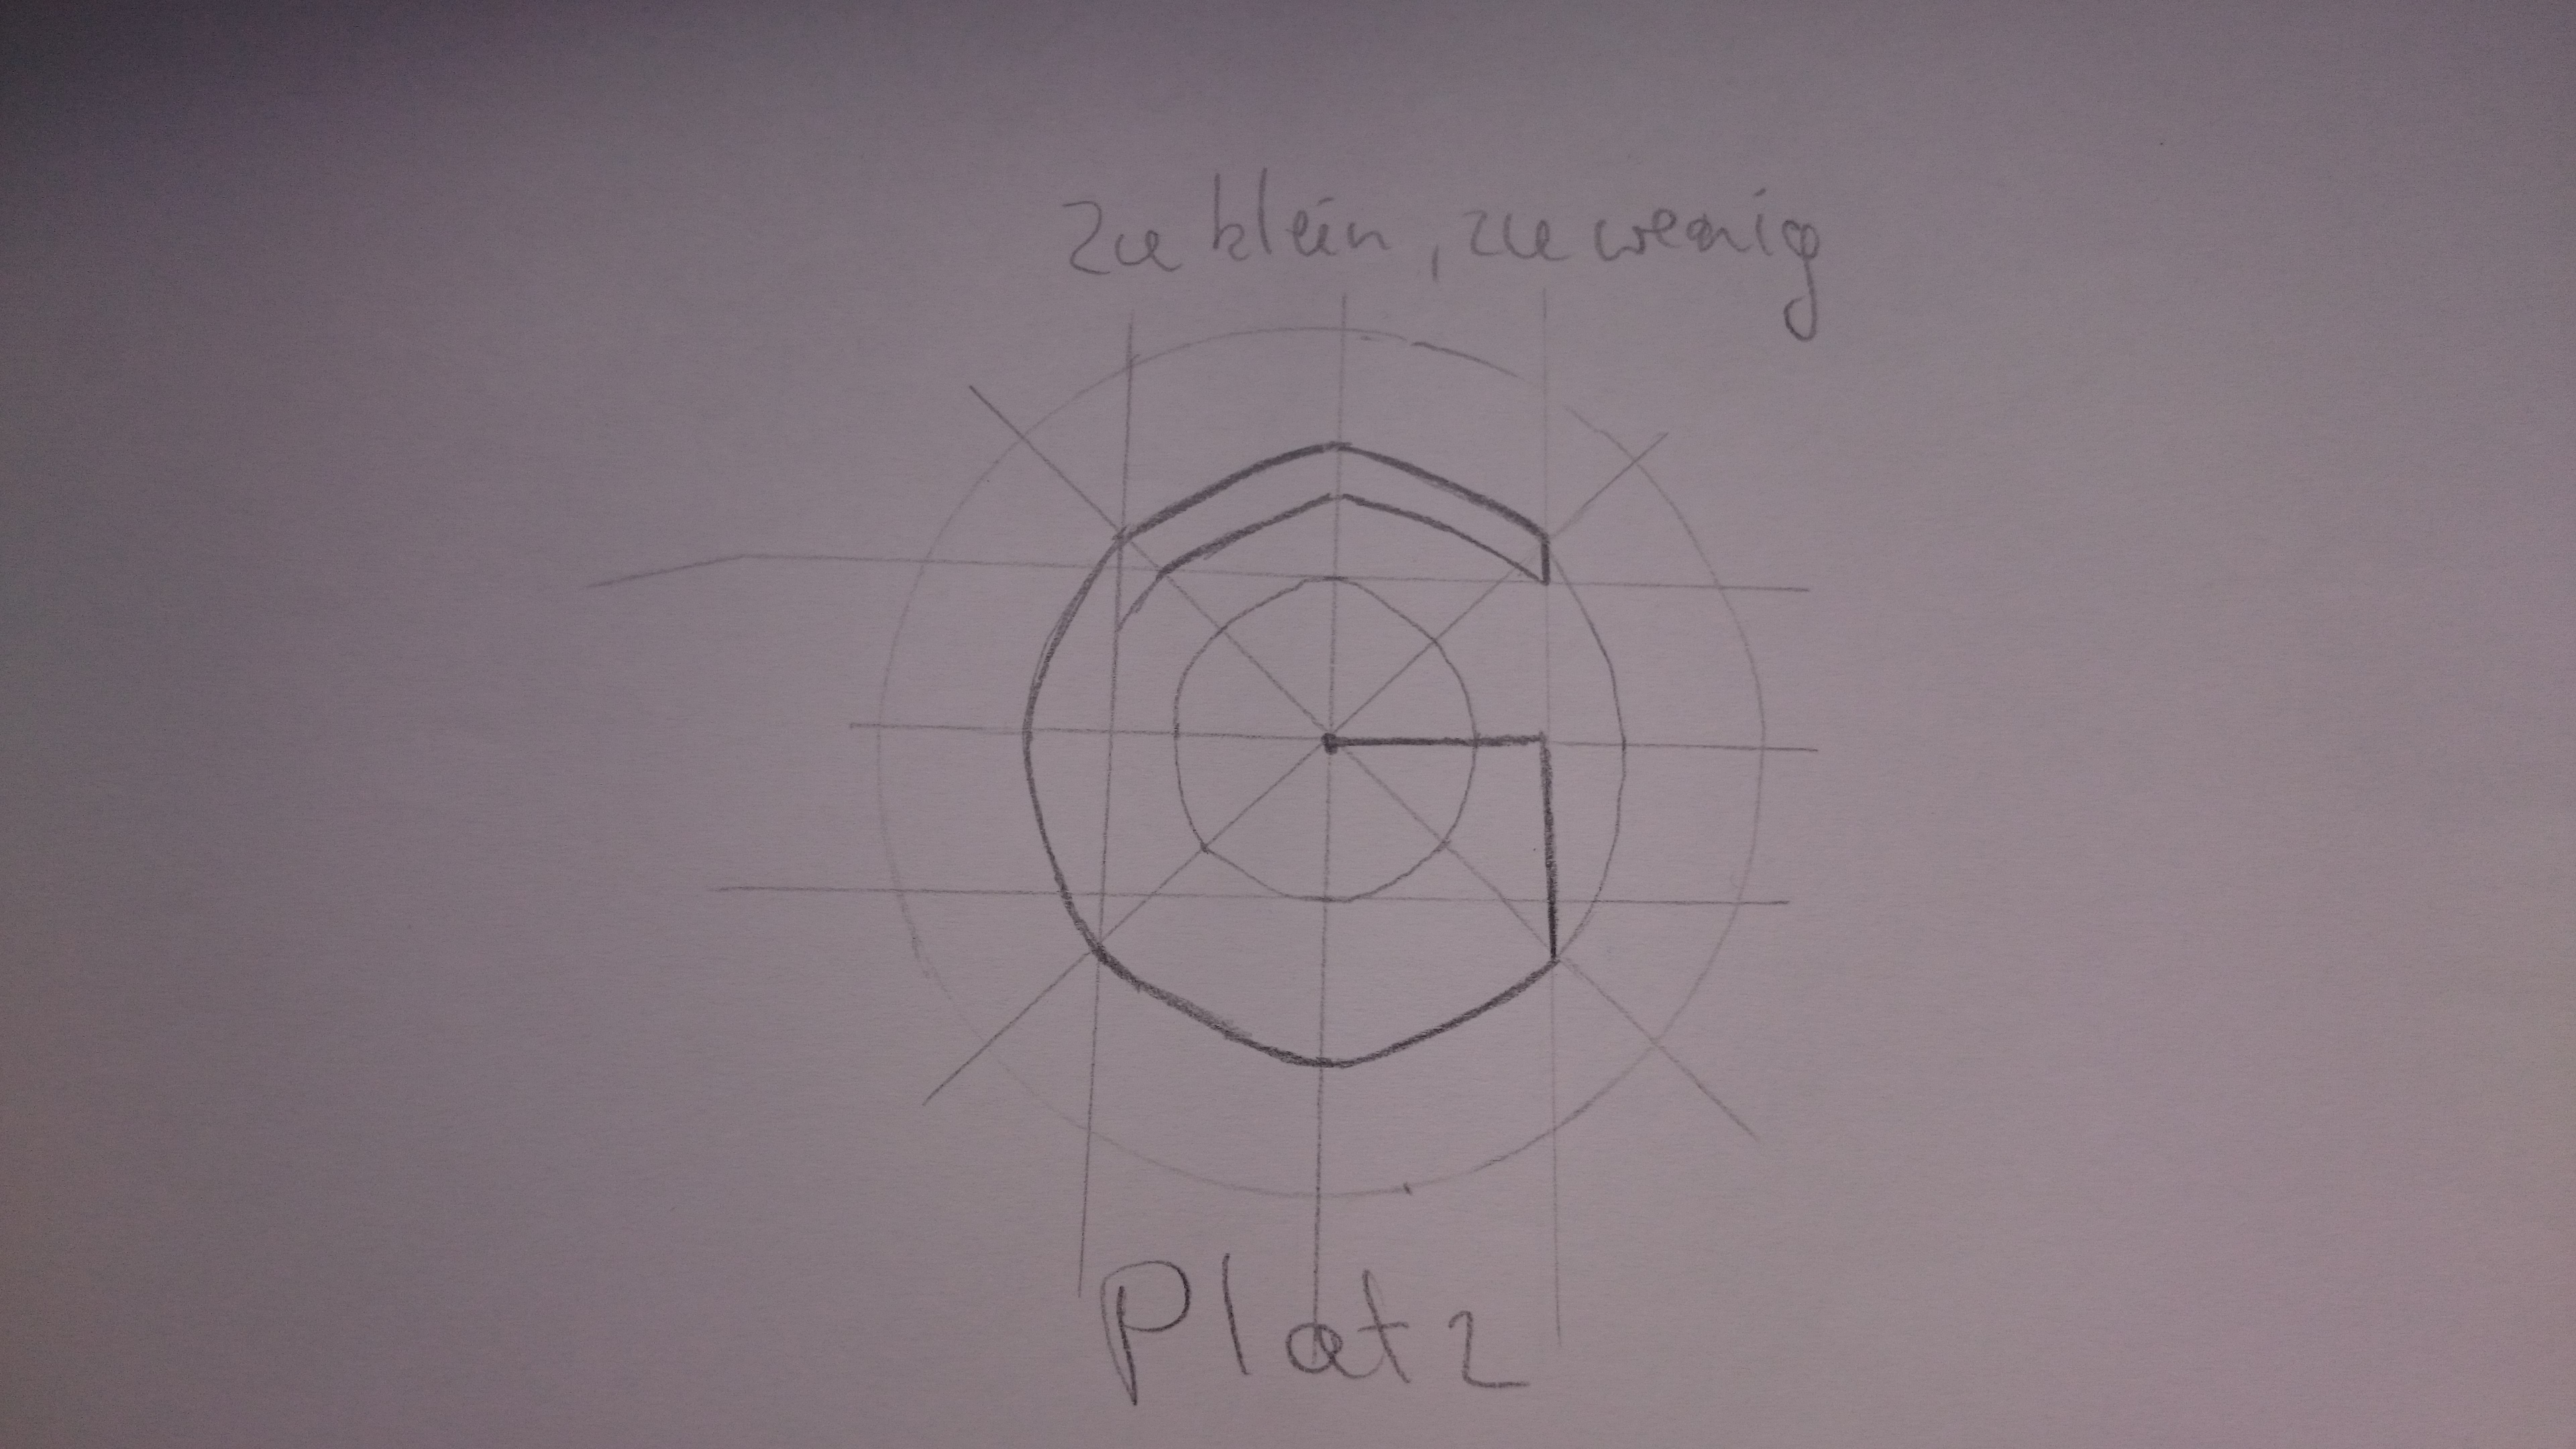
\includegraphics[scale=0.13]{DSC_0759.jpg}\\
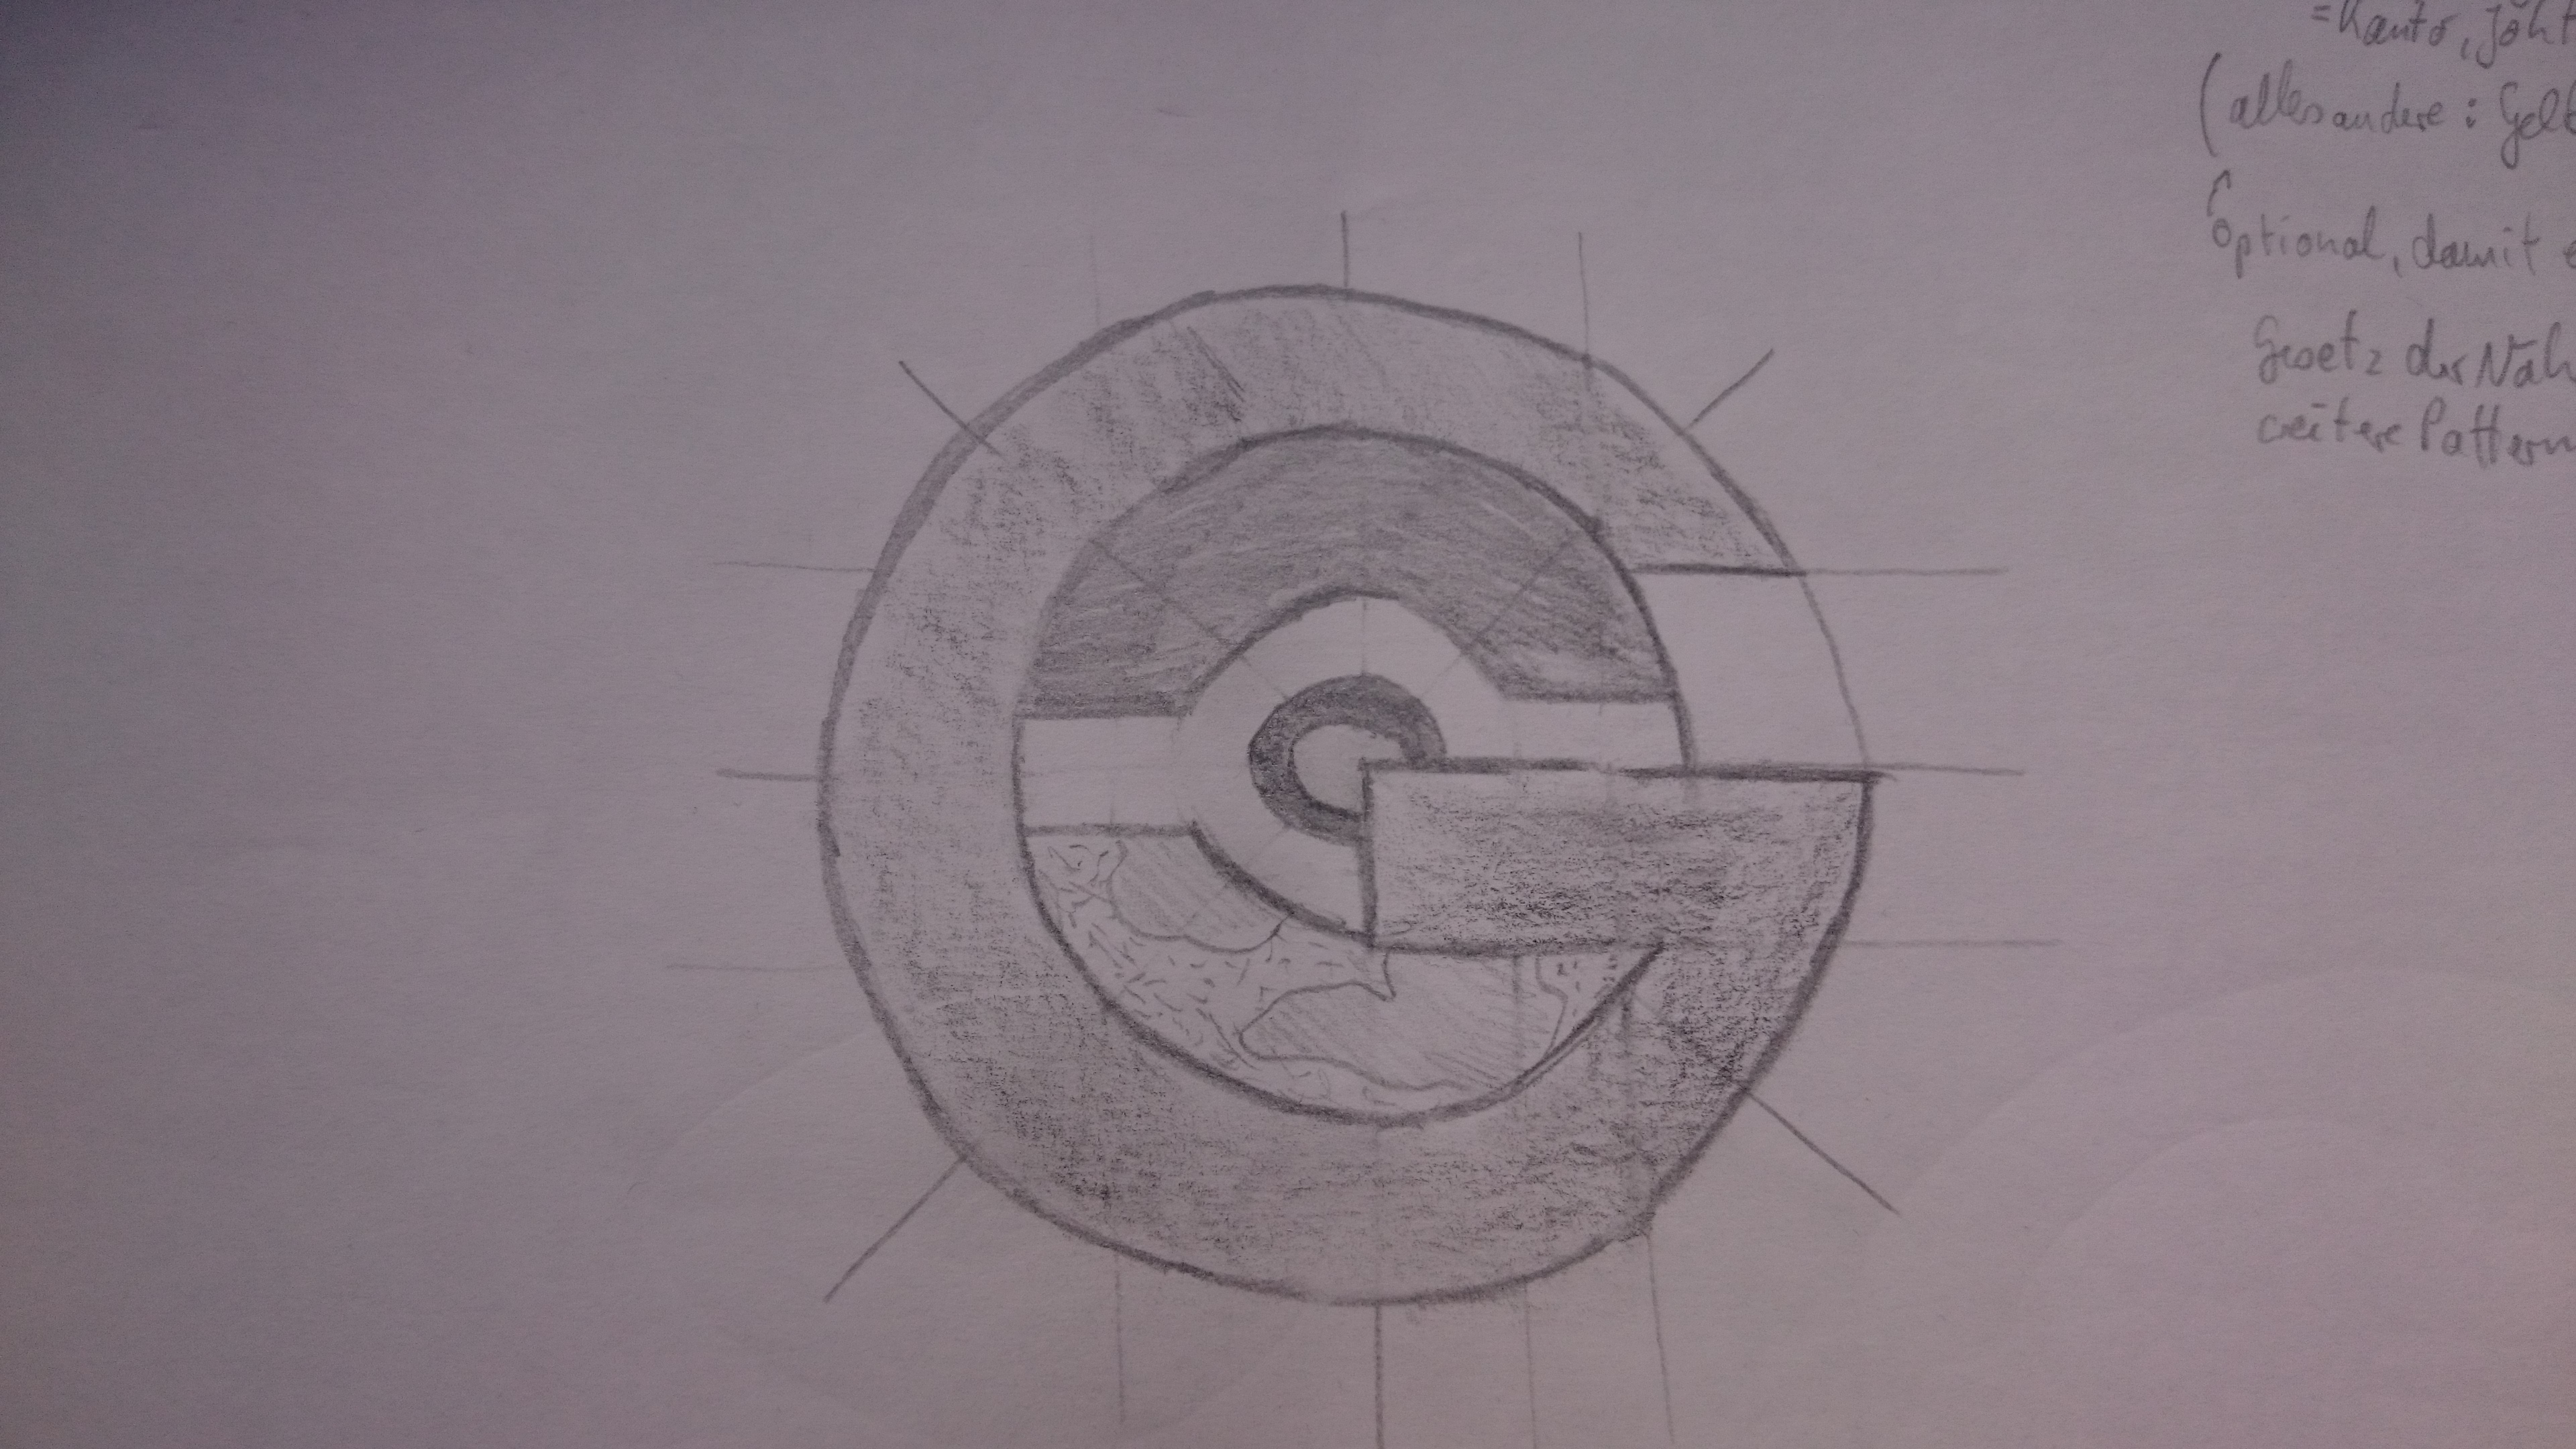
\includegraphics[scale=0.13]{DSC_0760.jpg}\\
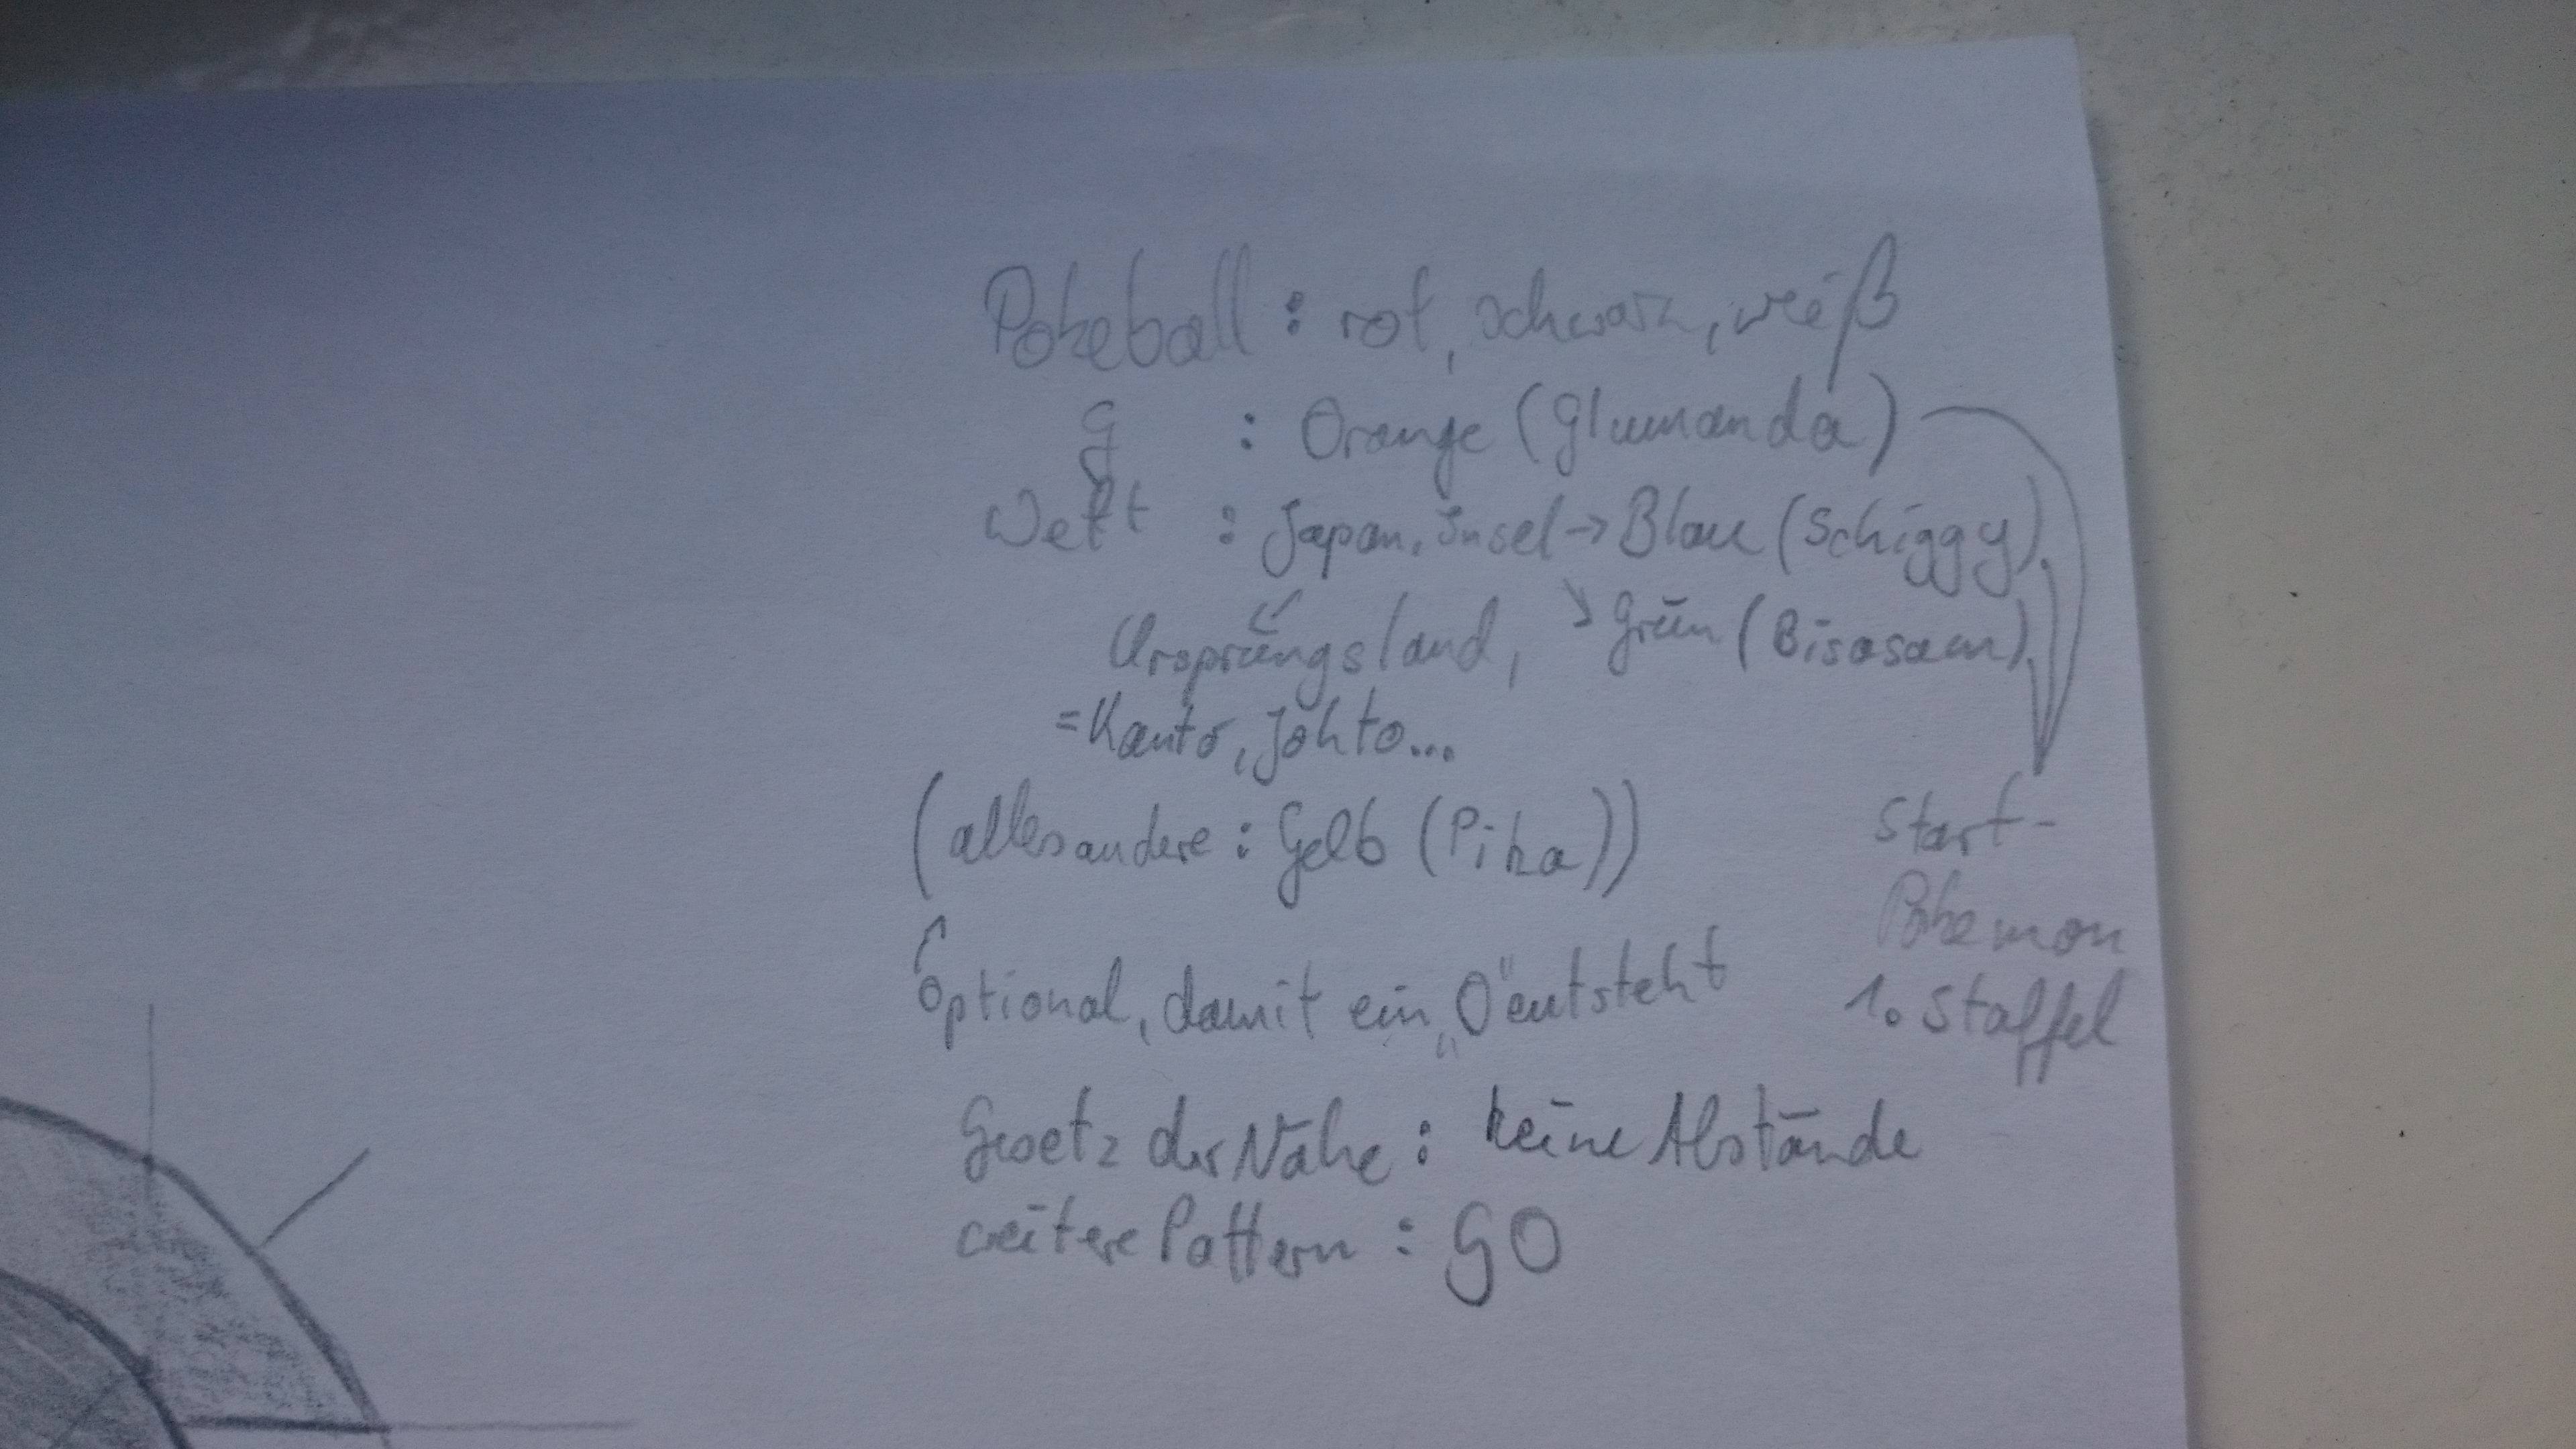
\includegraphics[scale=0.13]{DSC_0761.jpg}\\


 
\end{document}